\chapter{Overview of Flash-X architecture}
\label{Chp:Architecture}


The files that make up the Flash-X source are organized in the directory structure
according to their functionality and grouped into components called
\emterm{units}%\index{unit}.
Throughout this manual, we use the word `unit'
to refer to a group of related files that control a single aspect of a
simulation, and that provide the user with an interface of publicly 
available functions. Flash-X can be viewed as a collection of units, which
are selectively grouped to form one application.

A typical Flash-X simulation requires only a subset of all of the units in 
the Flash-X code. When the user gives the name of the simulation to the
\code{setup} tool, the tool locates and brings together the units required
by that simulation, using the Flash-X \code{Config} files (described in
\chpref{Chp:The Flash-X configuration script}) as a
guide. Thus, it is important to distinguish between the entire Flash-X 
source code and a given Flash-X application. 
the
Flash-X units can be broadly classified into five functionally distinct categories:
\emterm{infrastructure, physics, monitor, driver,}
and \emterm{simulation}.

The \emterm{infrastructure} category encompasses the units responsible for Flash-X housekeeping
tasks such as the management of runtime parameters, the handling of input and output
to and from the code, and the administration of the grid, which describes the simulation's
physical domain.

Units in the \emterm{physics} category such as \unit{Hydro} (hydrodynamics), \unit{Eos} (equation of state),
and \unit{Gravity} implement algorithms to solve the equations describing specific physical
phenomena. 

The \emterm{monitoring} units \unit{Logfile}, \unit{Profiler}, and \unit{Timers} track the progress of an
application, while the \unit{Driver} unit implements the time advancement methods and manages
the interaction between the included units.

The \emterm{simulation} unit is of particular significance because it defines how a Flash-X
application will be built and executed. When the setup script is invoked, it begins
by examining the simulation's \code{Config} file, which specifies the units required for
the application, and the simulation-specific runtime parameters. 
Initial conditions for the problem are provided in the routines \code{Simulation_init} and
\code{Simulation_initBlock}.
As mentioned in \chpref{Chp:Creating new problems}, the \unit{Simulation} unit allows the user
to overwrite any of Flash-X's default function implementations by writing a function with
the same name in the application-specific directory. Additionally, runtime parameters
declared in the simulation's \unit{Config} file override definitions of same-named parameters
in other Flash-X units. These helpful features enable users to
customize their applications, and are described in more detail below in
\secref{Sec:Inheritance} and online in %\tips{arch}{Architecture Tips}. 
The simulation unit also provides some useful interaces for modifying
the behaviour of the application while it is running. For example
there is an interface \code{Simulation\_adjustEvolution} which is
called at every time step. Most applications would use the null
implementation, but its implementation can be placed in the Simulation
directory of the application to customize behavior. The API functions
of the \code{Simulation} unit are unique in that except
\code{Simulation\_initSpecies}, none of them have any default general 
implementations. At the API level there are the 
null implementations, actual implementations exist only for specific 
applications. The general implementations of \code{Simulation\_initSpecies}
exist for different  classes of applications, such as those utilizing
nuclear burning or ionization. 

\begin{flashtip}
Why the name change from ``modules'' in \flashx to ``units'' in \flashx?
The term ``module'' caused confusion among users and developers because it could refer both
to a \FORTRAN 90 module and to the Flash-X-specific code entity. In order to avoid this problem, \flashx started using
the word ``module'' to refer exclusively to an \Fortran 90 module, and the word ``unit'' for the
basic Flash-X code component. Also, Flash-X no longer uses \Fortran 90 modules to implement
units.  Fortran's limitation of one file per module is too restrictive for some of
\flashx's units, which are too complex to be described by a single file. Instead, \flashx uses
interface blocks, which enable the code to take advantage of some of the advanced features of \FORTRAN 90,
such as pointer arguments and optional arguments. Interface blocks are used throughout the code,
even when such advanced features are not called for. For a given unit, the interface block will be supplied
in the file \code{"Unit_interface.F90"}. Please note that files containing calls to API-level functions
must include the line \code{use Unit, ONLY: function-name1, function-name2, etc.} at the top of the file.
\end{flashtip}

\section{Flash-X Inheritance}
\label{Sec:Inheritance}

\newcommand{\OS}{Unix\xspace}
\FORTRAN 90 is not an object-oriented language like Java or C++, and as such does not implement
those languages' characteristic properties of inheritance.  But Flash-X takes advantage of
the \OS directory structure to implement an inheritance hierarchy of its own. Every child
directory in a unit's hierarchy inherits all the source code of its parent, thus eliminating
duplication of common code. During setup, source files in child directories override same-named files in
the parent or ancestor directories.  

Similarly, when the
\code{setup} tool parses the source tree, it treats each 
child or subdirectory 
as inheriting all of the Config and Makefile files 
in its parent's directory. While source files at a given level of
the directory hierarchy override files with the same name at higher
levels, Makefiles and configuration files are
cumulative. 
Since functions can have multiple implementations,
selection for a specific application  follows a few simple rules
applied in order described in %\tips{arch}{Architecture Tips}.

However, we must take care that this special use of the directory structure for inheritance
does not interfere with its traditional use for organization. We avoid any problems by means
of a careful naming convention that allows clear distinction between organizational and
namespace directories. 

To briefly summarize the convention, which is described in detail
online in %\tips{arch}{Architecture Tips},
the
top level directory of a unit shares its name with that of the unit, and as such always begins with a
capital letter. Note, however, that the unit directory may not always exist at the top level of the source
tree. A class of units may also be grouped together
and placed under an organizational directory for ease of navigation; 
organizational directories are given in lower case letters.
For example the grid management
unit, called \unit{Grid}, is the only one in its class,
and therefore its path is \code{source/Grid}, whereas the hydrodynamics unit, \unit{Hydro}, is one of
several physics units, and its top level path is \code{source/physics/Hydro}. This method for
distinguishing between organizational directories and namespace directories is applied
throughout the entire source tree.



\section{Unit Architecture}
\label{Sec:Unit Architecture}

A Flash-X unit defines its own Application Programming Interface (API),
which is a collection of routines the unit exposes to other units in 
the code.  A unit API is usually a mix of accessor functions and
routines which modify the state of the simulation.

A good example to examine is the \unit{Grid} unit API. Some of the accessor
functions in this unit are \api{Grid/Grid_getCellCoords},
\api{Grid/Grid_getBlkData}, and \api{Grid/Grid_putBlkData}, 
while \api{Grid/Grid_fillGuardCells} and
\newline   % added to prevent overfull
\api{Grid/Grid_updateRefinement} are examples of API routines which
modify data in the \unit{Grid} unit.

A unit can have more than one implementation of its API.  The
\unit{Grid} Unit, for example, has both an \emterm{Adaptive Grid} and a
\emterm{Uniform Grid} implementation.  Although the implementations are
different, they both conform to the \unit{Grid} API, and therefore appear the
same to the outside units.  This feature allows users to easily swap 
various unit implementations in and out of a simulation without
affecting they way other units communicate.  Code does not have to be
rewritten if the users decides to implement the uniform grid instead
of the adaptive grid.  

\subsection{Stub Implementations}
Since routines can have multiple implementations, the \code{setup} script
must select the appropriate implementation for an application.
The selection follows a few simple rules described in
%\tips{arch}{Architecture Tips}.
The top directory of every unit
contains a \emterm{stub} or null implementation of each routine in the
Unit's API.  The stub functions essentially do nothing. They are coded
with just the declarations to provide the same interface to callers as
a corresponding ``real'' implementation. They act as function
prototypes for the unit. Unlike true prototypes, however,
the stub functions assign default values to the
output-only arguments, while leaving the other arguments
unaltered. The following snippet shows a simplified example of a stub
implementation for the routine \api{Grid/Grid_getListOfBlocks}.

\begin{shrink}
\begin{codeseg}
subroutine Grid_getListOfBlocks(blockType, listOfBlocks, count)

  implicit none

  integer, intent(in) :: blockType
  integer,dimension(*),intent(out) :: listOfBlocks
  integer, intent(out) :: count

  count=0
  listOfBlocks(1)=0

  return
end subroutine Grid_getListOfBlocks
\end{codeseg}
\end{shrink}

While a set of null implementation routines at the top level of
a unit may seem like an unnecessary added layer, this arrangement
allows Flash-X to include or exclude units without the need to modify any
existing code.  If a unit is not included in a simulation, the
application will be built with its stub functions. Similarly, if a
specific implementation of the unit finds some of the API functions
irrelevant, it need not provide any implementations for them.
In those situations, the applications include stubs for the
unimplemented functions, and full implementations of all the other
ones. Since the stub functions do return valid values when called,
unexpected crashes from un-initialized output arguments are avoided.

The \api{Grid/Grid_updateRefinement} routine is a good example of how
stub functions can be useful. In the case of a simulation using an
adaptive grid, such as \Paramesh, the routine \api{Driver/Driver_evolveFlash}
calls \code{Grid_updateRefinement} to update the grid's spacing. The Uniform
Grid however, needs no such routine because its grid is fixed.  There is no
error, however, when \code{Driver_evolveFlash} calls \code{Grid_updateRefinement}
during a Uniform Grid simulation, because the stub routine steps in and simply
returns without doing anything.  Thus the stub layer allows the same
\code{Driver_evolveFlash} routine to work with both the Adaptive Grid and
Uniform Grid implementations.


\begin{flashtip}
While the concept of ``null'' or ``stub'' functions existed in
\flashx, \flashx formalized it by requiring all units to 
publish their API (the complete Public Interface) at the top level of a
unit's directory. Similarly, the inheritance through \OS directory
structure in \flashx is essentially the same as that of Flash-X2,
but the introduction of a formal naming convention has clarified it
and made it easier to follow.
The complete API can be found online at \newline
\url{http://flash.uchicago.edu/site/flashcode/user_support/}.
\end{flashtip}

\subsection{Subunits}
One or more  %\index{\subunit}
\subunits sit under the top level of a unit.  
Among them the unit's complete API is implemented. The \subunits are
considered peers to one another.  Each \subunit must implement at
least one API function, and no two \subunits can implement the same
API function. The division of a unit into \subunits is based upon
identifying self-contained subsets of its API. In some instances, a
\subunit may be completely excluded from a simulation, thereby saving
computational resources. For example, the \code{Grid} unit API
includes a few functions that are specific to Lagrangian tracer particles, and
are therefore unnecessary to simulations that do not utilize
particles.  By placing these routines in the \code{GridParticles}
\subunit, it is possible to easily exclude them from a simulation.
The \subunits have composite names; the first part is the unit name,
and the second part represents the functionality that the \subunit
implements. The \emterm{primary \subunit}%\index{\subunit!primary}
is named \code{\metavar{Unit}Main},
which every unit must have. For example, the main \subunit of
\code{Hydro} unit is \code{HydroMain} and that of the \code{Eos} unit
is \code{EosMain}. 

In addition to the \subunits, the top level unit
directory may contain a subdirectory called \emph{localAPI}. This
subdirectory allows a \subunit to create a public interface to other
\subunits within its own unit; all stub implementations of the \subunit
public interfaces are placed in \code{localAPI}.   External units should \emph{not}
call routines listed in the \code{localAPI}; for this reason these
local interfaces are not shown in the general source API tree.

A \subunit can have a hierarchy of its own. It may have more than one
\uids with alternative implementations of some of its functions
while other functions may be common between them. 
Flash-X exploits the inheritance rules described in
% \tips{arch}{Architecture Tips}.
For example, the
\code{Grid} unit has three implementations for \code{GridMain}: the
Uniform Grid (UG), \Paramesh2, and \Paramesh4. The procedures to apply
boundary conditions are common to all three implementations, and are
therefore placed directly in \code{GridMain}. In addition, \code{GridMain} contains
two subdirectories.  One is \code{UG}, which has all the remaining
implementations of the API specific to the Uniform Grid. The other
directory is organized as \code{paramesh}, which in turn contains two directories
for the package of \Paramesh2 and another organizational directory \code{paramesh4}. 
Finally, \code{paramesh4} has two subdirectories with alternative implementations of
the \Paramesh4 package.
The directory \code{paramesh}
also contains all the function
implementations that are common between
\Paramesh2 and \Paramesh4.
Following the naming
convention described in %\tips{arch}{Architecture Tips},
\code{paramesh} is all lowercase, since it has child directories that
have some API implementation. The namespace directories \code{Paramesh2}, \code{Paramesh4.0} and\code{Paramesh4dev} contain functions 
unique to each implementation.  An example of a unit hierarchy is shown in
\figref{Fig:units_hierarchy}.  
The kernels are described below in \chpref{Sec:privateRoutines}.

\begin{figure}[ht] \begin{center}
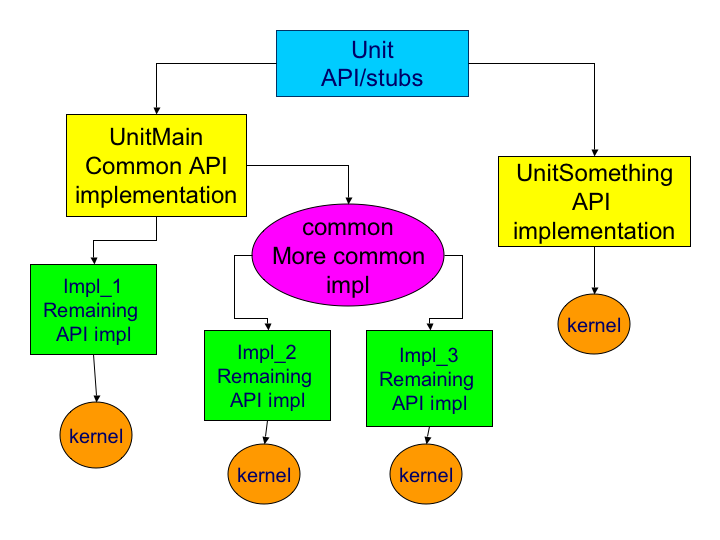
\includegraphics[width=5.0in]{arch_unit_heirarchy}
\caption{\label{Fig:units_hierarchy} The unit hierarchy and inheritance.}
\end{center} \end{figure} 

\subsection{Unit Data Modules, \code{_init}, and \code{_finalize} routines}
\label{Sec:Data Modules}

Each unit must have a \Fortran90 data module to store its unit-scope local data
and an \code{Unit\_init} file to initialize it. The \code{Unit\_init}
routines are called by the \unit{Driver} unit once by the routine
\api{Driver/Driver_initFlash} at the start of a simulation.  They get
unit specific runtime parameters from the
\unit{RuntimeParameters} unit and store them in the unit data module. 

Every \uid of \code{\metavar{Unit}Main}, must either inherit a
\code{\metavar{Unit}_data} module, or have its own. There is no
restriction on additional unit scope data modules, and individual
Units determine how best to manage their data. Other \subunits and the
underlying computational kernels can have their own data modules, but the developers are
encouraged to keep these data modules local to their \subunits and
kernels for clarity and maintainability of the code. It is strongly
recommended that only the data modules in the \code {Main} \subunit be
accessible everywhere in the unit. However, no data module of a unit
may be known to any other unit. This restriction is imposed to keep
the units encapsulated and their data private. If another part of the
code needs access to any of the unit data, it must do so through
accessor functions. 

Additionally, when routines use data from the unit's data module the
convention is to indicate what particular data is being used with the
\code{ONLY} keyword, as in
\code{use Unit\_data, ONLY : un\_someData}.  See the snippet of code
below for the correct convention for using data from a unit's \FORTRAN\
Data Module.
\begin{codeseg}
subroutine Driver_evolveFlash()

  use Driver_data, ONLY: dr_myPE, dr_numProcs, dr_nbegin, &
       dr_nend, dr_dt, dr_wallClockTimeLimit, &
       dr_tmax, dr_simTime, dr_redshift, &
       dr_nstep, dr_dtOld, dr_dtNew, dr_restart, dr_elapsedWCTime

  implicit none

  integer   :: localNumBlocks
\end{codeseg}

Each unit must also have a \code{Unit_finalize} routine to clean up the
unit at the termination of a Flash-X run.  The finalization routines might deallocate space
or write out completion messages.

\subsection{Private Routines:  kernels and helpers}
\label{Sec:privateRoutines}
All routines in a unit that do not implement the API are classified as
private routines. They are divided into two broad categories: the
\emph{kernel}%\index{kernel}
is the collection of routines that implement the unit's
core functionality and solvers, and \emph{helper} routines are
supplemental to the unit's API and sometimes act as a conduit
to its kernel. A helper function is allowed to know the other unit's
APIs but is itself known only locally within the unit. The concept of
helper functions allows minimization of the unit APIs, which assists in
code maintenance. The helper functions follow the
convention of starting with an  ``\code{un\_}'' in their name, where ``\code{un}'' is
in some way derived from the unit name. For example, the helper
functions of the \unit{Grid} unit start with \code{gr\_}, and those
of \unit{Hydro} unit start with \code{hy\_}. The helper functions
have access to the unit's data module, and they are also allowed to
query other units for the information needed by the kernel, 
by using their accessor functions. If the
kernel has very specific data structures, the helper functions can
also populate them with the collected information. An example of 
a helper function is \code{gr_expandDomain}, which refines an AMR block.
After refinement, equations of state usually need to be called, so the routine
accesses the EOS routines via \code{Eos_wrapped}.

The concept of
kernels, on the other hand, facilitates easy import of third party
solvers and software into  Flash-X. The kernels are not required to
follow either the naming convention or the inheritance rules of the
Flash-X architecture. They can have their own hierarchy and data
modules, and the top level of the kernel typically resides at leaf
level of the Flash-X unit hierarchy. This arrangement allows Flash-X to
import a solver without having to modify its internal code, since
API and helper functions hide the higher level details from it, and
hide its details from other units. However, developers
are encouraged to follow the helper function naming convention in the
kernel where possible to ease code maintenance. 

The \code{Grid} unit and the \code{Hydro} unit both provide very good
examples of private routines that are clearly distinguishable between
helper functions and kernel. The AMR version of the \unit{Grid} unit imports
the \Paramesh version 2 library as a vendor supplied branch in our repository. It
sits under the lowest namespace directory \code{Paramesh2} in \unit{Grid}
hierarchy and maintains the library's original structure. All other
private functions in the \code{paramesh} branch of \unit{Grid} are helper
functions and their names start with \code{gr\_}. In the \unit{Hydro} unit the
entire hydrodynamic solver resides under the directory \code{PPM},
which was imported from the PROMETHEUS code (see \chpref{Sec:PPM algorithm}). 
PPM is a directional
solver and requires that data be passed to it in vector form. Routines
like \code{hy\_sweep} and \code{hy\_block} are helper functions that
collect data from the \unit{Grid} unit, and put it in the format required by
PPM. These routines also make sure that data stay in thermodynamic
equilibrium through calls to the Eos unit. Neither \Paramesh2, nor PPM
has any knowledge of units outside their own. 



% \begin{flashtip}
% From a user's perspective, the most noticeable changes in architecture
% from \flashx to \flashx are related to the ownership and access to data.
% \flashx has a centralized database into which all the units (called
% modules in \flashx) register their data when the code is
% initialized. Modules query the central database for their data needs,
% including for the data that they themselves registered. \flashx, on the
% other hand has no central database.  Instead, units own their data
% and provide accessor/mutator functions for the data they are willing
% to share. For example, the \code{Grid} unit owns the data structures which
% represent variables on the physical grid. Various physics units need
% to operate on and modify this data as the solution evolves. Therefore, the
% \unit{Grid} unit provides a suite of \emterm{get} and \emterm{put} functions to access
% and modify the physical grid data. Similarly, time advancement related
% data such as
% \code{Dt} (timestep) and \code{simTime} (simulation time reached)
% belong to the \unit{Driver} unit, but most units need to use them. The
% \unit{Driver} unit provides \emterm{get} functions for \code{Dt} and \code{simTime}, but no
% \emterm{put} functions since no other unit should modify them.
% \newline
% Another change from \flashx is the introduction of the
% \code{Unit\_init} files which among other initializations read the
% runtime parameters for a particular unit.  In \flashx runtime
% parameters were initialized in \code{if(.firstcall.)}  blocks from
% anywhere in the code.  \flashx has streamlined these calls by having
% all of the runtime parameters relevant to a specific unit initialized
% once at the beginning of the simulation and stored in the
% \code{Unit\_data} Fortran module.
% \end{flashtip}






\section{Unit Test Framework}
\label{Sec: unitTest }
In keeping with good software practice, \flashx incorporates a unit
test framework that allows for rigorous testing and easy isolation of
errors. The components of the unit test show up in two different
places in the Flash-X source tree. One is a dedicated path in the
\code{Simulation} unit,
\code{Simulation/SimulationMain/\-unitTest/\metavar{UnitTestName}}, where 
\metavar{UnitTestName} is the name of a specific unit test. The other place is a
subdirectory called \code{unitTest}, somewhere in the hierarchy of the
corresponding unit which implements a function \fcn{Unit\_unitTest}
and any helper functions it may need. The primary reason for organizing unit
tests in this somewhat confusing way is that unit tests are special cases of 
simulation setups that also need extensive access to internal data of the unit
being tested. By splitting the unit
test into two places, it is possible to meet both requirements without
violating unit encapsulation. We illustrate the functioning of the
unit test framework with the unit test of the \unit{Eos} unit. For more
details please see \secref{Sec:Eos Unit Test}. The \unit{Eos} unit test needs its
own version of the routine \api{Driver/Driver_evolveFlash} which makes a
call to its \fcn{Eos\_unitTest} routine. The initial conditions
specification and unit test specific \fcn{Driver\_evolveFlash} are
placed in \code{Simulation/SimulationMain/unitTest/Eos}, since
the \unit{Simulation} unit allows any substitute Flash-X function to be placed in
the specific simulation directory. The function \code{Eos\_unitTest}
resides in \code{physics/Eos/unitTest}, and therefore has access to all
internal \unit{Eos} data structures and helper functions.

